\section{Integrale}

Integralrechnung ist das Gegenteil zur Ableitung

\begin{itemize}
    \item Ableitung: $f(x) = x^2+3 \rightarrow f'(x) = 2x$
    \item Integrieren: $f(x) = x^2+3 \leftarrow f'(x) = 2x$
    \item $F(x) = \frac{2x^2}{2} = x^2+c$ wobei $c \in \mathbb{R}$        $\mathbb{R}$ ist die Integrationskonstante
    \item Stammfunktion = $\textcolor{red}{F(x)}$
    \item Algemein: $f(x) = c^n \rightarrow \textcolor{red}{F(x)} = \frac{x^{n+1}}{n+1}+c$
\end{itemize}

Man benötight eine Zusatzinformation um die Stammfunktion bcw.: $c$ eindeutig bestimmen zu können.

\hfill \break
\subsection{Anwändung Inigral}

Die Integralrechnung wird verwendetum...\\
\begin{itemize}
    \item um die Tammfuntion zu bestimmen $\rightarrow$ Das bestimmte Integral
    \item um die Fläche unter einer Funtion zu bestimmen $\rightarrow$ Das unbestimmte Integral
\end{itemize}
\break
\newpage
\subsection{Das bestimmte Integral}

Die Ableitung der Stammfunktion ergibt die Funktion selbst. $\rightarrow F'(x)=f(x)$

\hfill\break
\begin{itemize}
    \item Bestimme die Stammfunktion der Funktion $f(x)=2x$
    \item Welche Funktion ergibt abgeleitet $f(x)=2x \rightarrow F(x)=x^2$
    \item Weil $\rightarrow F'(x) = 2x = f(x)$
\end{itemize}

Eine Ableitungsregel besagt, dass eine Konstante beim Ableiten wegfällt.
Aus diesem Grund ist die oben angegebene Lösung nur eine von unendlich vielen, denn auch z.B. $F(x)=x^2+3$ und $F(x)=x^2-9$ sind Stammfunktionen von $f(x)=2x$.
Da sich die einzelnen Stammfunktionen nur durch eine Konstante $C$ unterscheiden, schreiben wir $F(x)=x^2+C$
\break
\newpage
\subsection{Das unbestimmte Integral}

Die Fläche wird immer von Nullstelle zu Nullstelle berechnet weil wen man versucht die rechn ung auf einmal
mit den taschenrechner zu lösen wird alles unter dem Nullpunkt von allem größer null subtrahieren.


$$A=\int\limits_1^7 3dx=3x+c |_1^7 = \textcolor{red}{3*7+x}-\textcolor{blue}{(3*1+c)} = 21-3 = 18$$
\begin{itemize}
    \item \textcolor{red}{obere Gänze}
    \item \textcolor{blue}{unterre Gänze}
\end{itemize}


\hfill \break
Example:\\
\fboxrule=0.8pt \fcolorbox{lightgray}{lightgray}{%
    \begin{tabular}{ |c|}
        \hline
        GrundFormel: $f(x) = -x^2+4$                                                                                                                                                                \\
        $F(x) = -\frac{x^3}{3} +4x$                                                                                                                                                                 \\
        Integral: $\int\limits_{-2}^2 f(x)dx$                                                                                                                                                       \\
        $\int\limits_{-2}^2 f(x)dx = 2*\int\limits_0^2 f(x)dx = 2*(-\frac{x^2}{3}+4 |_0^2) = 2*(\frac{2}{3}+4*2(-\frac{0^3}{3}+4*0)=2*(-\frac{8}{3}+8) = 2* \frac{16}{3} = \frac{32}{3})$ \\
        \hline
    \end{tabular}}\\

\hfill \break
\begin{itemize}
    \item Gegben: $f(x)=3$
    \item Gesucht: Flächeninhalt ($f(x)$) von $x_1=1$ bis $x_2=7$
\end{itemize}


\hfill \break
Mit dem Taschenrechner: Rechnerrisch:
\begin{enumerate}
    \item Math $\uparrow$
    \item a: fnInt
    \item fnint(3,x,\textcolor{red}{1},\textcolor{blue}{7}) $\textcolor{red}{1=x_1}$ $\textcolor{blue}{7=x_2}$
\end{enumerate}

\hfill \break
Mit dem Taschenrechner: Grafisch:
\begin{enumerate}
    \item $y_1$ = 3
    \item $2_{nd}$ calc 7. f(x)dx
\end{enumerate}


\break
\newpage
\subsection{Fläche zwischen Funktionen}

Es soll die Fläche zwischen den beiden Funktionen ermittelt werden:
\begin{itemize}
    \item $\textcolor{blue}{f(x) = x^2+2}$
    \item $\textcolor{red}{g(x) = -x^2+5}$
\end{itemize} 

\hfill \break
Schritte:
\begin{enumerate}
    \item Schnittpunkte Berechnen: \begin{itemize}
        \item Ermittlung durch Gleichsetzen: $f(x) = g(x)$
        \item Ermittlung mit TR $2_{nd}$ calc intersect
    \end{itemize}
    \item Zwischen den ermittelten Schnittpunkten Integrieren: $\int\limits_{x2}^{x1} g(x)-f(x)dx$
\end{enumerate}

\hfill \break
Dabei sit zu beachten das immer die obere minus der unterren Kurve gerechnet werden muss.

\hfill \break
Example:\\
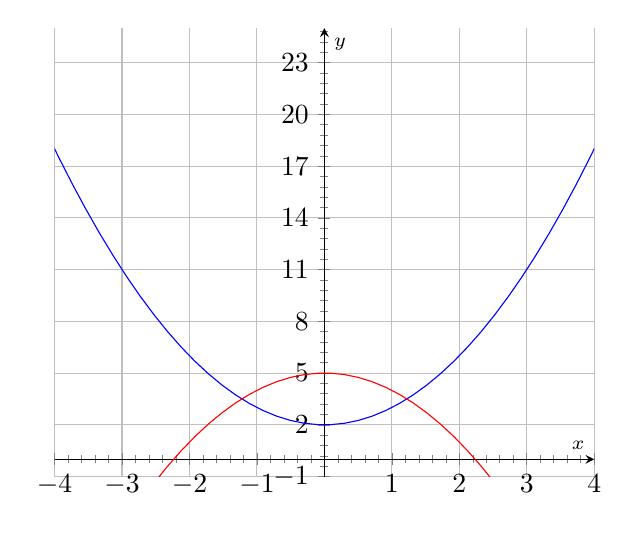
\begin{tikzpicture}[scale=1]
    \begin{axis}%
        [
            grid=major,
            xtick={-5,-4,...,4},
            minor x tick num=4,
            xmin=-4,
            xmax=4,
            xlabel={\scriptsize $x$},
            axis x line=middle,
            ytick={-1,2,...,25},
            minor y tick num=4,
            ymin=-1,
            ymax=25,
            ylabel={\scriptsize $y$},
            axis y line=middle,
            no markers,
            samples=100,
            domain=-10:10,
        ]
        \addplot[blue] (x,{x^2+2});
        \addplot[red] (x,{-x^2+5});
    \end{axis}
\end{tikzpicture}
\break
\newpage
\subsection{Kurvenschar}

Eine Kurvenschar ergiebt sich darurch das das $c$ bein intigreieren nicht bestimmt ist: $f(x)dx = F(x)+c$.\\
Und da $c \in \mathbb{R}$ wegeben sich verschiedene Möglichkeiten für $c$ was sin in den möglichen Kurven wiederspiegelt.

\hfill \break
Example:\\
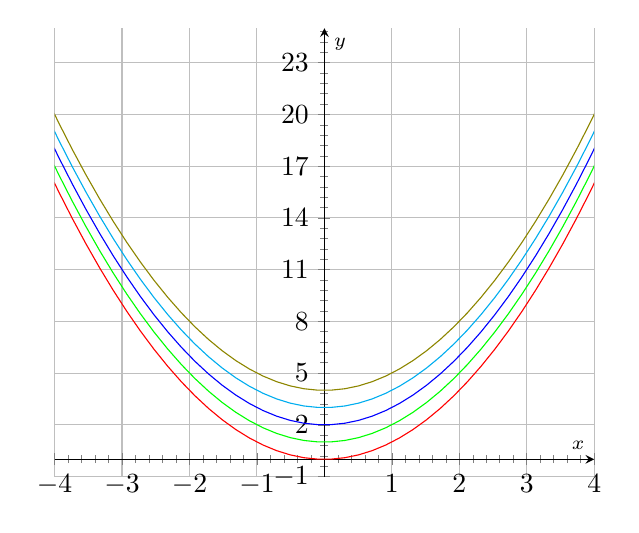
\begin{tikzpicture}[scale=1]
    \begin{axis}%
        [
            grid=major,
            xtick={-5,-4,...,4},
            minor x tick num=4,
            xmin=-4,
            xmax=4,
            xlabel={\scriptsize $x$},
            axis x line=middle,
            ytick={-1,2,...,25},
            minor y tick num=4,
            ymin=-1,
            ymax=25,
            ylabel={\scriptsize $y$},
            axis y line=middle,
            no markers,
            samples=100,
            domain=-10:10,
        ]
        \addplot[red] (x,{x^2+0});
        \addplot[green] (x,{x^2+1});
        \addplot[blue] (x,{x^2+2});
        \addplot[cyan] (x,{x^2+3});
        \addplot[olive] (x,{x^2+4});
    \end{axis}
\end{tikzpicture}
